\documentclass[a4paper]{article}
\usepackage[utf8]{inputenc}
\usepackage[spanish, es-tabla, es-noshorthands]{babel}
\usepackage[table,xcdraw]{xcolor}
\usepackage[a4paper, footnotesep = 1cm, width=22cm, top=2.5cm, height=25cm, textwidth=20cm, textheight=25cm]{geometry}
%\geometry{showframe}

\usepackage{tikz}
\usepackage{amsmath}
\usepackage{amsfonts}
\usepackage{amssymb}
\usepackage{float}
\usepackage{graphicx}
\usepackage{caption}
\usepackage{subcaption}
\usepackage{multicol}
\usepackage{multirow}
\usepackage{wrapfig}
\setlength{\doublerulesep}{\arrayrulewidth}
\usepackage{booktabs}

\usepackage{hyperref}
\hypersetup{
    colorlinks=true,
    linkcolor=blue,
    filecolor=magenta,      
    urlcolor=blue,
    citecolor=blue,    
}

\newcommand{\note}[1]{
	\begin{center}
		\huge{ \textcolor{red}{#1} }
	\end{center}
}

\setcounter{topnumber}{2}
\setcounter{bottomnumber}{2}
\setcounter{totalnumber}{4}
\renewcommand{\topfraction}{0.85}
\renewcommand{\bottomfraction}{0.85}
\renewcommand{\textfraction}{0.15}
\renewcommand{\floatpagefraction}{0.8}
\renewcommand{\textfraction}{0.1}
\setlength{\floatsep}{5pt plus 2pt minus 2pt}
\setlength{\textfloatsep}{5pt plus 2pt minus 2pt}
\setlength{\intextsep}{5pt plus 2pt minus 2pt}

\newcommand{\quotes}[1]{``#1''}
\usepackage{array}
\newcolumntype{C}[1]{>{\centering\let\newline\\\arraybackslash\hspace{0pt}}m{#1}}
\usepackage[american]{circuitikz}
\usetikzlibrary{calc}
\usepackage{fancyhdr}
\usepackage{units} 

\graphicspath{{../Ejercicio-1/}{../Ejercicio-2/}{../Ejercicio-3/}{../Ejercicio-4/}{../ParteI/}{../ParteII/}{../ParteIII/}{../ParteIV/}}

\pagestyle{fancy}
\fancyhf{}
\lhead{22.14 - Electrónica IV}
\rhead{Mechoulam, Lambertucci, Londero}
\rfoot{Página \thepage}


\begin{document}

\subsection{Introducción}

Se analizó la conmutación de un MOSFET \href{https://www.vishay.com/docs/91019/91019.pdf}{IRF530} de potencia en un circuito con carga inductiva, utilizando un diodo \href{https://www.onsemi.com/pdf/datasheet/mur420-d.pdf}{MUR460} de potencia para proporcionar un camino a la corriente durante el apagado del MOSFET y no dañar al circuito.

%Aca puede ir la foto del circuito

Para la conmutación del MOSFET se utilizó un periodo de $T_s = 20 \mu s$ y un duty cycle de $D = 50 \%$.

\subsection{Circuito en la Teoría}

En la teoría, se consideró al diodo IRF530 como ideal excepto por la caída de potencial de la juntura en directa, siendo esta extraída de la datasheet, con un valor de $V_{D_{on}} = 1.3V$. Además, se consideró a la bobina como ideal con resistencia serie nula.

\begin{figure}[H]
	\centering
	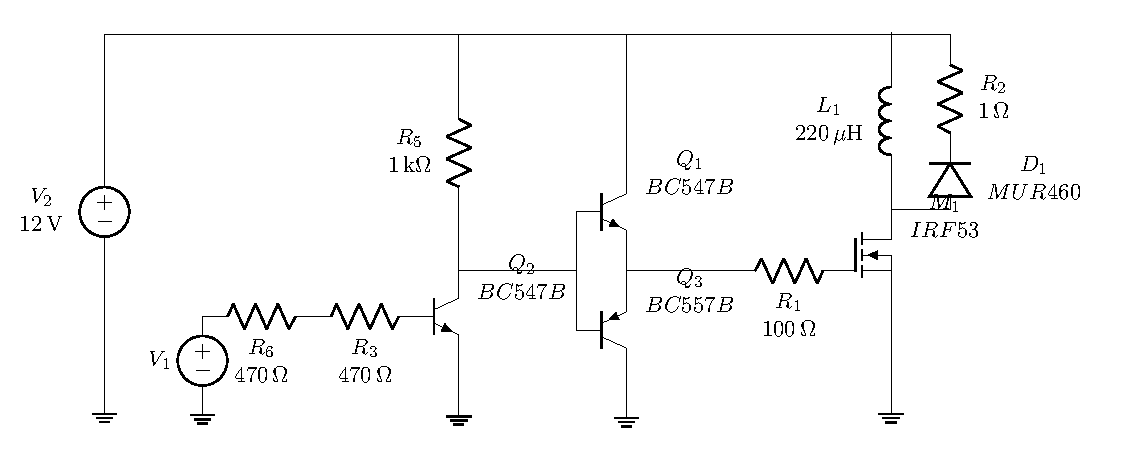
\includegraphics[width=0.7\linewidth, page=1]{ImagenesEjercicio-1/CircuitsEj1}
	\caption{Circuito para el estudio de la conmutación del MOSFET.}
	\label{fig:ej1:circuito}
\end{figure}

\subsubsection{Primer Hemicircuito: MOSFET ON}

Cuando el MOSFET se encuentra encendido, y despreciando la caída $V_{ds_{on}}$ entre drain y source, la bobina posee una tensión de $V_{L_{on}} = V_i = 12V$ entre sus bornes, por lo que la corriente $I_L$ que la atraviesa crece de manera constante a razón de $\frac{V_i}{L} = \frac{12V}{220\mu H}$. Como el diodo se encuentra con su ánodo conectado a tierra, y su cátodo conectado a $V_i$, este se encuentra en inversa por lo que no circula corriente a través de él.

\begin{figure}[H]
	\centering
	\includegraphics[width=0.4\linewidth, page=3]{ImagenesEjercicio-1/CircuitsEj1}
	\caption{Hemicircuito con MOSFET encendido.}
	\label{fig:ej1:circuito_on}
\end{figure}

\subsubsection{Segundo Hemicircuito: MOSFET OFF}

Una vez apagado el MOSFET, la bobina posee la tensión $V_{L_{off}}$ necesaria entre sus bornes para que siga circulando la corriente $I_L$, por lo que sobre el MOSFET caen $V_{ds_{off}} = V_i - V_{L_{off}}$ (tener en cuenta que ahora $V_{L_{off}} < 0$). En este estado, toda la corriente $I_L$ de la bobina pasan por el diodo el cual se encuentra polarizado en directa a consecuencia de la tensión impuesta por la bobina. No se extrae corriente de la fuente de alimentación en este estado si se desprecia la corriente parásita del MOSFET.

\begin{figure}[H]
	\centering
	\includegraphics[width=0.4\linewidth, page=2]{ImagenesEjercicio-1/CircuitsEj1}
	\caption{Hemicircuito con MOSFET encendido.}
	\label{fig:ej1:circuito_off}
\end{figure}

\subsubsection{Análisis de los Tiempos de Conmutación: Encendido}

Al encender el MOSFET con un escalón de tensión en $V_{GG}$, tomado en el borne izquierdo de $R_1$, crece la corriente de gate $I_G$ instantáneamente a un valor de $I_G = \frac{V_i}{R_1} = 0.12A$ para luego decrecer exponencialmente según (\ref{eq:ej1:ig_ton}). Al mismo tiempo, la tensión entre gate y source pasa de ser nula a crecer exponencialmente según (\ref{eq:ej1:vgs_ton}).

\begin{equation}
I_G(t) = -\frac{V_{GG}}{R_1}e^{-\frac{t}{\tau_1}}
\label{eq:ej1:ig_ton}
\end{equation}

\begin{equation}
V_{gs}(t) = V_{GG}(1-e^{-\frac{t}{\tau_1}})
\label{eq:ej1:vgs_ton}
\end{equation}

\subsection{Circuito en la Simulación}

\subsection{Circuito en la Práctica}

\subsection{Diferencias}

\subsection{Conclusiones}

\end{document}